\newcommand{\om}{\Omega}
\renewcommand{\a}{\mathcal{A}}
\newcommand{\f}{\mathcal{f}}


%Chargement des paquets
\usepackage{amsmath}
\usepackage{amsfonts}
\usepackage{amssymb}
\usepackage{enumerate}
\usepackage{mathtools}
\usepackage{bbm}
\usepackage{xparse, etoolbox}
\usepackage{enumerate}
\usepackage{enumitem}
\usepackage{mathabx}
\usepackage{babel}[french]

%environment
\usepackage{amsthm}
\usepackage{keytheorems}
\usepackage{hyperref} 

%Interface théorème
\newkeytheorem{lem}[
	name = Lemme
]

\newkeytheorem{prop}[
	name = Proposition
]

\newkeytheorem{thm}[
	name = Théorème
]

\newkeytheorem{coro}[
	name = Corollaire
]

\renewcommand*{\proofname}{Démonstration}

\theoremstyle{definition}
\newtheorem{defn}{Définition}

\theoremstyle{definition}
\newtheorem*{nota}{Notation}

\theoremstyle{definition}
\newtheorem*{limi}{Liminaire}

\theoremstyle{remark}
\newtheorem{rmq}{Remarque}

\theoremstyle{plain}
\newtheorem*{fait}{Fait}


%Ensembles de nombres
\newcommand{\N} {\mathbb{N}}
\newcommand{\Ne}{\N^\ast}
\newcommand{\Z} {\mathbb{Z}}
\newcommand{\Q} {\mathbb{Q}}
\newcommand{\R} {\mathbb{R}}
\newcommand{\Rb}{\overline{\mathbb{R}}}
\newcommand{\Rp}{\R_+}
\newcommand{\Rm}{\R_-}
\newcommand{\K} {\mathbb{K}}
\newcommand{\Ket} {\mathbb{K^{\ast}}}
\newcommand{\Cx}{\mathbb{C}}

%Ensembles, tribus
\newcommand{\A}{\mathbb{A}}
\renewcommand{\P}{\mathcal{P}}
\newcommand{\T}{\mathcal{T}}
\newcommand{\F}{\mathcal{F}}
\newcommand{\C} {\mathcal{C}}
\newcommand{\ouv}{\mathcal{O}}
\newcommand{\B}{\mathcal{B}}
\newcommand{\M}{\mathcal{M}}
\newcommand{\etag}{\mathcal{E}}
\newcommand{\etagOp}{\etag^{+}(\Omega)}
\newcommand{\etagO}{\etag(\Omega)}
%%Lp avant quotientage
\newcommand{\Lic}{\mathcal{L}^1}
\newcommand{\Lpc}{\mathcal{L}^p}
\newcommand{\Linfc}{\mathcal{L}^{\infty}}
\newcommand{\Lifull}{\Lic(\Omega, \B, m)}
\newcommand{\Lpfull}{\Lpc(\Omega, \B, m)}
\newcommand{\Linffull}{\Linfc(\Omega, \B, m)}
%%Lp après quotientage
\newcommand{\Li}{L^1}
\newcommand{\Ld}{L^2}
\newcommand{\Lp}{L^p}
\newcommand{\Linf}{L^{\infty}}
\newcommand{\Listd}{\Li(\Omega, m)} 
\newcommand{\Ldstd}{\Ld(\Omega, m)} 
\newcommand{\Lpstd}{\Lp(\Omega, m)} 

%Quelques opérateurs
\DeclareMathOperator{\codim}{codim}
\DeclareMathOperator{\rg}{rg}
\DeclareMathOperator{\tr}{tr}
\DeclareMathOperator{\vect}{Vect}
\DeclareMathOperator{\ima}{Im}
\DeclareMathOperator{\id}{Id}
\DeclareMathOperator{\sign}{sign}
\DeclareMathOperator{\ext}{ext}
\newcommand{\ind}{\mathbbm{1}}
\newcommand*{\spr}[2]{\left(\,#1\,\middle|\,#2\,\right)}
\newcommand{\interior}[1]{%
  {\kern0pt#1}^{\mathrm{o}}%
}
\DeclareMathOperator{\card}{card}
\DeclareMathOperator{\ppcm}{ppcm}

%Commandes de pure flemme
\newcommand{\veps}{\varepsilon}
\newcommand{\intab}{\int_{a}^{b}}
\newcommand{\intR}{\int_{-\infty}^{\infty}}
\newcommand{\intinf}{\int_{- \infty}^{+ \infty}}
\newcommand{\equi}{\Leftrightarrow}
\newcommand{\Kev}{$\K$-espace vectoriel }
\newcommand{\Kevs}{$\K$-espaces vectoriels }
\newcommand{\Rev}{$\R$-espace vectoriel }
\newcommand{\Revs}{$\R$-espaces vectoriels }
\newcommand{\Cev}{$\Cx$-espace vectoriel }
\newcommand{\Cevs}{$\Cx$-espaces vectoriels }
\newcommand{\evn}{(E, \norm{.})}
\newcommand{\interf}[2]{[#1,#2]}
\newcommand{\limb}{\lim\limits_}
\newcommand{\lebn}{\lambda_n}
\newcommand{\pp}{\text{~presque partout}}
\newcommand{\derivp}[2]{\frac{\partial #1}{\partial #2}}
\newcommand{\famiu}{(u_i)_{i \in I}}
\newcommand{\sev}{\text{~s.e.v.}}
\newcommand{\Mnp}{M_{n,p}(\K)}
\newcommand{\Mn}{M_{n}(\K)}
\newcommand{\tq}{\text{~t.q.~}}
\newcommand{\mq}{~montrer~que~}
\newcommand{\et}{\quad \text{et} \quad}
\newcommand{\ou}{\text{~ou~}}
\newcommand{\Kx}{\K[X]}


%Commandes de gars chelou
\renewcommand{\subset}{\subseteq}

%Commande restriction, ty duckduckgo
\def\restr#1#2{\mathchoice
              {\setbox1\hbox{${\displaystyle #1}_{\scriptstyle #2}$}
              \restraux{#1}{#2}}
              {\setbox1\hbox{${\textstyle #1}_{\scriptstyle #2}$}
              \restraux{#1}{#2}}
              {\setbox1\hbox{${\scriptstyle #1}_{\scriptscriptstyle #2}$}
              \restraux{#1}{#2}}
              {\setbox1\hbox{${\scriptscriptstyle #1}_{\scriptscriptstyle #2}$}
              \restraux{#1}{#2}}}
\def\restraux#1#2{{#1\,\smash{\vrule height .8\ht1 depth .85\dp1}}_{\,#2}} 

%Quelques normes
\DeclarePairedDelimiter\abs{\lvert}{\rvert}
\DeclarePairedDelimiter\labs{\bigl\lvert}{\bigr\rvert}
\DeclarePairedDelimiter\norm{\lVert}{\rVert}
\DeclarePairedDelimiterXPP\normi[1]{}\lVert\rVert{_1}{\ifblank{#1}{\:\cdot\:}{#1}}
\DeclarePairedDelimiterXPP\normd[1]{}\lVert\rVert{_2}{\ifblank{#1}{\:\cdot\:}{#1}}
\DeclarePairedDelimiterXPP\normp[1]{}\lVert\rVert{_p}{\ifblank{#1}{\:\cdot\:}{#1}}
\DeclarePairedDelimiterXPP\normq[1]{}\lVert\rVert{_q}{\ifblank{#1}{\:\cdot\:}{#1}}
\DeclarePairedDelimiterXPP\norminf[1]{}\lVert\rVert{_\infty}{\ifblank{#1}{\:\cdot\:}{#1}}

%Bracket en angle
\DeclarePairedDelimiter\angl{\langle}{\rangle}

%Set, parenthèses
\newcommand{\set}[1]{\{ #1 \}}
\newcommand{\bigset}[1]{\bigl\{ #1 \bigr\}}
\newcommand{\Bigset}[1]{\Bigl\{ #1 \Bigr\}}
\newcommand{\bigpar}[1]{\bigl( #1 \bigr)}
\newcommand{\Bigpar}[1]{\Bigl( #1 \Bigr)}

%Opitmisation des opérateurs de comparaison
\DeclarePairedDelimiter\tio{o (}{)}
\DeclarePairedDelimiter\gro{O (}{)}


\pagestyle{fancy}

\fancyhead[C]{Le processus de Galton-Watson}
\fancyhead[R]{}

\begin{document}

\section{Positionnement du problème}

\underline{Problématique :} dynamique d'une population issue d'un individu. \\

\underline{Situation historique :} transmission d'un nom de famille (système patrilinéaire ou matrilinéaire strict). \\

\begin{nota}
On note $n \in \N$ le compteur générationel. \\
La variable $Z_n$ représente le nombre d'individus à la génération $n$, $Z_0 = 1$. \\
A chaque génération, un individu donne naissance à un certains nombre d'individus puis est considéré mort à la génération suivante. \\
On suppose que la loi du nombre de descendants est la même pour chaque individu, et que ce nombre est indépendant de la
descendance des autres individus. \\
On note $X$ la variable aléatoire discrète à valeurs dans $\N$ donnant le nombre de descendants d'un individu d'une génération 
donnée et $P(X=k) = p_k$. \\
On introduit la suite double $(X_i^n)$ de variables aléatoires indépendantes de même loi que $X$ et on considère que, 
à la génération $n$, l'individu $i$ (parmi les $Z_n$) engendrera $X_i^n$ descendants. \\
Ainsi, à la génération $n+1$, le nombre total d'individus sera égal à :
\[ Z_{n+1} = \sum_{i=1}^{Z_n} X_i^n . \] 
On suppose que tous les $X_i^n$ admettent un moment d'ordre 1 , et on note :
\[ m = E[X] \] 
On pose :
\[ G(t) = E[t^X] = \sum_{n=0}^{\infty} p_n t^n , \]
la fonction génératrice des $X_i^n$. Enfin, on note $x_n = P \set{Z_n = 0}$, i.e. la probabilité que la population s'éteigne à la génération
$n$. \\
On remarque que l'évènement \og M : la population finit par s'éteindre \fg{} est l'union croissante des évènements 
$\set{Z_n = 0} ; n \geq 0$ soit, par $\sigma$-additivité :
\[ P(M) = \lim_{n \to \infty} x_n . \]
Enfin, si $p_0 = 1$, alors la population s'éteind dès la génération 1, on supposera donc dans la suite que $p_0 \neq 1$.
\end{nota}

\section{Résultats préalables}

\begin{thm}[Fubini-Tonelli]
Soient $(X, \a, m)$ et $(Y, \a', m')$ deux espaces mesurés tels que les deux mesures sont $\sigma$-finies et soit 
$(X \times Y, \a \times \a', m \times m')$ l'espace mesuré produit muni de la mesure produit. Si
\[ f : X \times Y \to [0, \infty] \]
est une application $\a \times \a'$-mesurable, alors les applications 
\[ x \mapsto \int_Y f(x,y) dm'(y) \et y \mapsto \int_X f(x,y) dm(x) \]
sont respectivement $\a$ et $\a'$-mesurables et :
\[ \int_{X \times Y} f(x,y) d(m\times m')(x, y) = \int_X \left ( \int_Y f(x,y) dm'(y) \right) dm(x) 
= \int_Y \left( \int_X f(x,y) dm(x) \right ) dm(y) . \]
\end{thm}

\begin{lem}
On suppose que $p_0 \neq 1$, la fonction génératrice $G$ est :
\begin{enumerate}[label=(\alph*)]
\item bien définie et de classe $\C^1$ sur $[0,1]$ ;
\item strictement croissante sur $]0,1[$ ;
\item convexe sur $]0,1[$ ;
\item si de plus $p_0+p_1<1$, $G$ est strictement convexe sur $]0,1[$.
\end{enumerate}
\end{lem}

\begin{proof}
\begin{enumerate}[label=(\alph*)]
\item La série entière $\sum p_n t^n$ a un rayon de convergence au moins égal à 1, $G$ est donc de classe $\C^{\infty}$ sur $]-1, 1[$.
En particulier, comme $X$ admet un moment d'ordre 1, $G'(1) = m < \infty$ ce qui montre que $G$ est de classe $\C^1$ sur $[0,1]$.
\item Il existe $k \geq 1$ tel que $p_k > 0$ donc $G'(t) \geq k p_k t^{k-1} > 0$. 
\item Si $k=1$ alors $G''=0$ et sinon $G''(t) \geq k(k-1) p_k t^{k-1} > 0$.
\item Si de plus $p_0+p_1 < 1$, alors il existe $k \geq 2$ tel que $p_k > 0$ et $G''(t) \geq k(k-1) p_k t^{k-2} > 0$.
\end{enumerate}
\end{proof}

\begin{thm}
Pour $n \in \N$, la fonction génératrice $G_n$ de $Z_n$ vérifie la relation de récurrence :
\[ G_{n+1} = G_n \circ G . \]
\end{thm}

\begin{proof}
La variable $Z_n$ et les variables $X_i^n$ sont mutuellement indépendantes (ce qui revient à affirmer que le nombre d'enfants d'un
individu de la génération $n$ est indépendant du nombre d'individus de cette même génération). \\
La probabilité que $Z_{n+1}$ soit égale à un entier $q$ est :
\begin{align*}
P\set{Z_{n+1} = q} & = \sum_{k=0}^{\infty} P \left \{ \sum_{i=1}^{Z_n} X_i^n = q ; Z_n = k \right \} \\
& = \sum_{k=0}^{\infty} P\left \{ \sum_{i=1}^k X_i^n = q ; Z_n = k \right \} \\
& = \sum_{k=0}^{\infty} P\left \{ \sum_{i=1}^k X_i^n = q \right \} P\set{Z_n=k},
\end{align*}
par indépendance des variables $X_i^n$ et $Z_n$. Donc, pour $t \in [-1, 1]$ :
\begin{align*}
G_{n+1}(t) & = \sum_{q=0}^{\infty} P \set{Z_{n+1} = q} t^q \\
& = \sum_{q=0}^{\infty} \sum_{k=0}^{\infty} P\left \{ \sum_{i=1}^k X_i^n = q \right \} P\set{Z_n=k} t^q \\
& = \sum_{k=0}^{\infty} \sum_{q=0}^{\infty} P\left \{ \sum_{i=1}^k X_i^n = q \right \} P\set{Z_n=k} t^q \qquad \text{(Fubini)} \\
& = \sum_{k=0}^{\infty} P\set{Z_n=k} \sum_{q=0}^{\infty} P\left \{ \sum_{i=1}^k X_i^n = q \right \} t^q \\
& = \sum_{k=0}^{\infty} P\set{Z_n=k} E[t^{\sum_{i=1}^k X_i^n}] ,
\end{align*}
Or, les $X_i^n$ étant mutuellement indépendants, on a $E[t^{\sum_{i=1}^k X_i^n}] = (G(t))^k$, soit :
\begin{align*}
G_{n+1}(t) & = \sum_{k=0}^{\infty} P\set{Z_n=k} G(t)^k \\
& = G_n(G)
\end{align*}
\end{proof}

\section{Exctinction de la population}

Puisque $G_0=\id$, on en déduit que :
\[ G_1 = G \et G_n = \underbrace{G \circ \cdots \circ G}_{\textit{n fois}} . \]
De plus, comme $x_n = P \set{Z_n=0} = G_n(0)$, on en déduit le théorème ci-dessous.

\begin{thm}
La suite $(x_n)_\N$ est caractérisée par sa valeur initiale $x_0=0$ et par la relation de récurrence :
\[ x_{n+1} = G(x_n) . \]
Notamment, la suite $(x_n)_\N$ converge, et sa limite $\alpha$ est égale à la plus petite racine de l'équation $G(x) = x$ sur $[0,1]$.
\end{thm}

\begin{proof}
La relation de récurrence est une conséquence directe du théorème précédent. \\
La fonction $G$ est croissante sur $[0,1]$, $G(0) \in [0,1]$ et $G(1) = 1$ donc l'intervalle $[0,1]$ est stable par $G$ 
et $G$ admet un point fixe en 1.
Notons $a$ le plus petit point fixe de $G$ sur $[0,1]$. \\
Si $G(0)=0$ alors $a=0$ et la suite est constante et égale à 0. Dans ce cas, la population ne s'éteind jamais. \\
Sinon, $G(0) > 0$ et, par croissance de $G$ on a $G([0,a]) \subset [0,a]$. De plus, par continuité de $G$ on a 
\[ \forall x \in [0, a[, G(x) > x \]
(sinon $G-\id$ s'annule, par continuité, en un point $x_0<a$). \\
Ainsi, la suite $(x_n)_\N$ est à valeurs dans $[0,a]$ et est croissante, donc elle converge. Par continuité, elle converge donc vers un point
fixe de $G$ ce qui montre que $a = \alpha$.
\end{proof}

On sait que la fonction $G$ admet au moins un point fixe : 1. Si ce point fixe est unique, la population s'éteind de façon certaine en 
vertue du théorème précédent. Mais il existe d'autres cas. Pour les étudier, on note $m=G'(1)=E(X)$ et on pose :
\[ \begin{array}{c c c c}
f : & [0,1] & \to & \R \\
& t & \mapsto & \left \{ \begin{array}{c c} \dfrac{G(t)-1}{t-1} & \text{ si } t < 1 \\ m & \text{ sinon} \end{array} \right.
\end{array} . \]
$f$ est continue sur $[0,1]$ (car $G$ est dérivable sur $[0,1]$). De plus, comme $G$ est convexe (resp. strictement) sur $]0,1[$, 
$f$ est croissante (resp. strictement) sur ce même intervalle ce qui permet de déduire les résultats suivants : 

\begin{enumerate}
\item \textbf{$m<1$}, pour tout $t \in [0,1[, f(t) \leq m$ donc $G(t) - 1 \geq m(t-1)$ 
soit $G(t)-t \geq (t-1)(m-1) > 0$, donc 1 est le seul point fixe de $G$ et la population s'éteind presque sûrement.
On dit que le système est sous-critique. 

\item \textbf{$m=1$}, le système est dit critique et il faut distinguer plusieurs sous-cas.

\begin{enumerate}
\item si $p_0 + p_1 = 1$, i.e. les individus donnent presque sûrement naissance à au plus un seul enfant, comme 
$m = E(X) = 1$ on en déduit que $p_1 = 1$ et $G=\id$, la population ne s'éteind jamais ;
\item sinon $p_0 + p_1 < 1$ donc $G$ est strictement convexe sur $]0,1[$ et $f$ est strictement croissante sur $]0,1[$. \\
Donc $\forall t \in [0,1[, G(t) - t > 0$ et 1 est le seul point fixe de $G$. La population s'éteind presque sûrement.
\end{enumerate}

\item \textbf{$m>1$}, par continuité de $f$, on peut trouver $t_0 \in [0,1[$ tel que 
$f(t_0) > 1$ soit $G(t_0) - t_0 < 0$. Or $G(0) \geq 0$ donc la fonction $G$ admet un point fixe sur $[0,1[$. 
De plus, le cas $G(0)=0$ est exclu car alors $G = \id$ et $G'(1) = 1$ ce qui viole l'hypothèse sur $m$. 
Le plus petit point fixe de $G$ est donc un élément de $]0,1[$ et l'exctinction de la population n'est pas certaine. \\
On dit que le système est sur-critique.
\end{enumerate}

Les représentations graphiques des différents cas sont données ci-dessous :

\begin{multicols}{3}

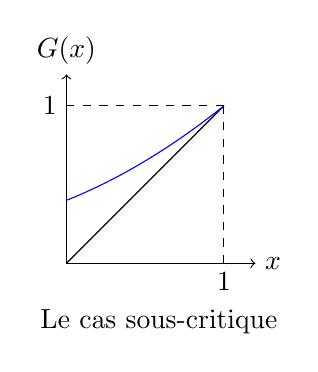
\begin{tikzpicture}[domain=0:1,scale=2]
  \draw[->] (-0,0) -- (1.2,0) node[right] {$x$};
  \draw[->] (0,0) -- (0,1.2) node[above] {$G(x)$};

  \draw[color=black]    plot (\x,\x);
  \draw[color=blue]   plot (\x, 2/5 + 2/5*\x + 1/5*\x^2);
  
  \node[below] at (1,0) {1};
  \node[left] at (0,1) {1};
  \draw[dashed] (1,0) -- (1,1);
  \draw[dashed] (1,1) -- (0,1);
  \node[below] at (current bounding box.south) {Le cas sous-critique};
\end{tikzpicture}

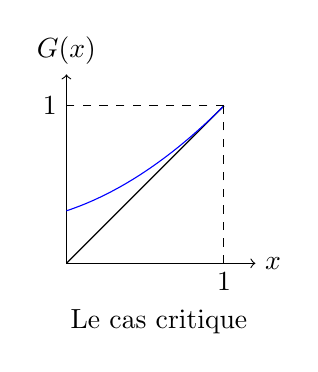
\begin{tikzpicture}[domain=0:1,scale=2]
  \draw[->] (-0,0) -- (1.2,0) node[right] {$x$};
  \draw[->] (0,0) -- (0,1.2) node[above] {$G(x)$};

  \draw[color=black]    plot (\x,\x);
  \draw[color=blue]   plot (\x, 1/3 + 1/3*\x + 1/3*\x^2);
  
  \node[below] at (1,0) {1};
  \node[left] at (0,1) {1};
  \draw[dashed] (1,0) -- (1,1);
  \draw[dashed] (1,1) -- (0,1);
  \node[below] at (current bounding box.south) {Le cas critique};
\end{tikzpicture}

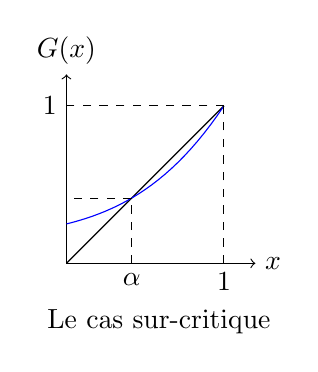
\begin{tikzpicture}[domain=0:1,scale=2]
  \draw[->] (-0,0) -- (1.2,0) node[right] {$x$};
  \draw[->] (0,0) -- (0,1.2) node[above] {$G(x)$};

  \draw[color=black]    plot (\x,\x);
  \draw[color=blue]   plot (\x, 1/4 + 1/4*\x + 1/4*\x^2 + 1/4*\x^3);
  
  \node[below] at ({sqrt(2)-1},0) {$\alpha$};
  \draw [dashed] ({sqrt(2)-1},0) -- ({sqrt(2)-1},{sqrt(2)-1});
  \draw [dashed] ({sqrt(2)-1},{sqrt(2)-1}) -- (0, {sqrt(2)-1});
  
  \node[below] at (1,0) {1};
  \node[left] at (0,1) {1};
  \draw[dashed] (1,0) -- (1,1);
  \draw[dashed] (1,1) -- (0,1);
  \node[below] at (current bounding box.south) {Le cas sur-critique};
\end{tikzpicture}

\end{multicols}

\section{Evolution de la population}
Comme $G(1) = 1$ et que $G_{n+1} = G_n \circ G$ on démontre aisément que :
\[ G'_{n+1}(1) = G'(1) \cdot G'_n(G(1)) = m G'_n(1) , \]
Or $E(Z_n) = G_n'(1)$ donc, par récurrence, on déduit que ;
\[ E(Z_n)=m^n . \]

Par conséquence :
\begin{enumerate}
\item dans le cas sous-critique, la population moyenne tend rapidement vers 0 ;
\item dans le cas critique, la population moyenne reste constante ;
\item dans le cas sur-critique, la population moyenne explose rapidement vers $\infty$.
\end{enumerate}

\newpage

\section{Annexe}

\subsection{Quelques bases}

Pour les résultats probabilistes, $\om$ désigne l'univers des possibles. 
On muni $\om$ d'une tribu $\a$ ainsi que d'une mesure finie $p$ sur  $(\om, \a)$ vérifiant $p(\om)=1$. 
Cette mesure $P$ est une mesure de probabilité et on dit que $(\om, \a, P)$ est un espace probabilisé. 
A noter qu'un univers muni d'une tribu est un espace probabilisable.

\begin{lem}
Pour une mesure $m$ quelconque sur un espace mesurable $(\om, \a)$, l'axiome de $\sigma$-additivité est équivalent au suivant : \\
Pour toute famille croissante $(B_n)_\N$ d'éléments de $\a$, on a :
\[ m \left( \bigcup_{n=0} ^{\infty} B_n \right ) = \lim_{n \to \infty} m(B_n) \]
\end{lem}

\begin{proof}
On revient à la $\sigma$-additivité en posant $A_n = B_n \setminus B_{n-1}$ et $B_{-1} = \emptyset$.
\end{proof}

\begin{defn}
Soit $(\om, \a)$ un espace probabilisable, une famille d'évènements de $\a$ est un système exhaustif (ou complet) si ces évènements
sont deux à deux disjoints et si leur réunion est l'univers tout entier. \\
Dans un espace probabilisé $(\om, \a, P)$, un système quasi-exhaustif (ou quasi-complet) d'évènements de $\a$ est, 
de façon simillaire, une famille d'évènements deux à deux disjoints et dont la probabilité de la réunion est 1
(l'union des évènements est quasi-certaine).
\end{defn}

\begin{defn}[Variable aléatoire]
Soient $(\om, \a, p)$ un espace probabilsé et $(E, \f)$ un espace probabilisable. 
On appelle variable aléatoire de $\om$ vers $E$ une application $X : \om \to E$ telle que $\forall F \in \f, X^{-1}(F) \in \a$.
La fonction $P_x : \f \to [0,1], F \mapsto P(X^{-1}(F))$ est alors une mesure de probabilité sur $(E, \f)$, appelé loi de probabilité de $X$.
\end{defn}

\begin{rmq}
Une loi de probabilité est dite discrète si $X(\Omega)$ est au plus dénombrable.
\end{rmq}

\begin{nota}
Pour une variable aléatoire $X$ à valeurs dans $\N$ on note $p_n = P(X=n)$
\end{nota}

\begin{lem}
Si $(B_i)_I$ est un système quasi complet d'évènements, et si $A$ est un évènement, alors :
\[ P(A) = \sum_{i \in I} P(A \cap B_i) . \] 
\end{lem}

\begin{proof}
Il suffit de considérer $\om = \bigcup B_i \cup \om \setminus \bigcup B_i$ avec $om \setminus \bigcup B_i$ un évènement de 
probabilté nulle.
\end{proof}

\begin{defn}[Moment]
Soit $p \geq 1$ et $X$ une variable aléatoire discrète réelle sur $\o$, on dit que $X$ admet un moment d'ordre $p$ lorsque
$X^p$ est sommable. On appelle alors moment d'ordre $p$ la valeur :
\[ E(X^p) = \sum_{x \in X(\om)} x^p P(X=x) . \]
\end{defn}

\begin{lem}
La série entière $\sum p_n t^n$ converge normalement sur $[-1,1]$ et a un rayon de convergence au moins égal à 1.
\end{lem}

\begin{proof}
On remarque que $\forall t \in [-1, 1], \abs{p_n t^n} \leq p_n$ et $\sum_{\N} p_n = 1$, d'où la convergence normale. \\
Comme de plus la suite $(p_n)_\N$ est bornée le rayon de convergence est bien au moins égal à 1.
\end{proof}

\begin{defn}[Série génératrice]
Soit $X : \om \to \N$ une variable aléatoire. On appelle série génératrice de $X$ ma série entière notée $G_X(t)$ et définie par :
\[ G_X(t) = \sum_{n=0}^{\infty} p_n t^n . \]
\end{defn}

\begin{lem}
Pour $t \in [0,1]$, on a $G_X(t) = E(t^X)$.
\end{lem}

\begin{proof}
Conséquence du théorème de transfert.
\end{proof}

\end{document}
